\section{Круги Эйлера}
\fontsize{12}{10}
\begin{center}
	\color{red}$(A \cup B) \setminus (A \cap B)$
\end{center}
\begin{center}
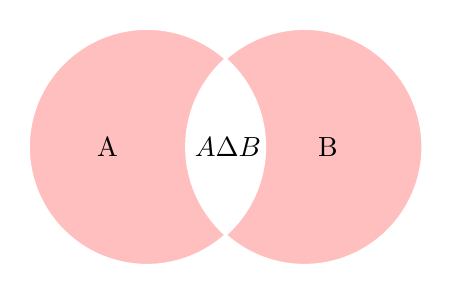
\begin{tikzpicture}[thick,
	set/.style = {circle,
		minimum size = 3cm,
		fill= pink}]

	\node[set] (A) at (0,0) {};
	\node[set] (B) at (2,0) {};
	
	\begin{scope}
		\clip (0,0) circle(1.5cm);
		\clip (2,0) circle(1.5cm);
		\fill[white] (0,0) circle(1.5cm);
	\end{scope}

	\draw[white] (0,0) circle(1.5cm);
	\draw[white] (2,0) circle(1.5cm);	
	\node at (-0.5,0) {A};
	\node at (2.3,0) {B};
	\node at (1.03,0) {$A\Delta B$};
	
\end{tikzpicture}
\end{center}
\begin{center}
Рис. 1: Симметрическая разность
\end{center}
